\chapter{Evaluation} \label{evaluation}
This chapter discusses the evaluation of \textit{qbftoepr} starting with the automated testing then benchmarks against other \gls{qbf} solvers and against \textit{qbf2epr}, a tool that also converts \gls{qbf} to \gls{epr}.

\section{Automated Testing}
Automated testing was implemented using the OUnit library which is an OCaml analogue of JUnit for Java. Each function was tested individually against valid and invalid inputs to determine whether the code behaved correctly then linked together in integration tests to test the sections of the algorithm (such as Skolemization) from the top level. Each update to the code also updated the tests if required and ensured that the tests passed before the code was committed.

\section{Testing Methodology}
Two test sets were selected from the QBFLIB 2010 problem library. The first was an easy set consisting of four easier problems with fewer clauses and the second was a more difficult set of sixteen harder problems with orders of magnitude more clauses. The exact problems are listed in appendix~\ref{qbfproblemsets}.

The easy set was used to test \textit{qbftoepr} against the \gls{qbf} solver DepQBF. The problems generated by the harder set were not practical to solve using iProver due to time constraints. This will become evident when comparing the iProver solving time of results generated using the trivial dependency scheme versus the standard in subsection~\ref{tvsstdsolve}. The easy set of benchmarks runs quickly enough to be able to benchmark efficiently but is complex enough to still provide a useful benchmark.

The hard set is used when evaluating the different dependency schemes and when comparing \textit{qbftoepr} to \textit{qbf2epr}. The solving time of iProver doesn't matter when comparing the two \gls{epr} converters because they produce the same result (ignoring differences in naming of variables and predicates) so a harder data set can be used to really challenge the converters.

The tests were run on a mid-2014 Macbook Pro with an Intel Core i7-4578U processor and 16GB of 1600MHz RAM running OS X El Capitan version 10.11.4. Each benchmark was ran three times to take an average.

\section{Comparison Between Trivial and Standard Dependency Schemes} \label{trivialvsstd}
Because the implementation of the standard scheme is inefficient it is expected to take much longer to convert the \gls{qbf} than the trivial scheme. The real benefits of the standard scheme are shown in the size of the outputted \gls{epr} result as a smaller output from the same input indicates the variable dependencies that were removed. This small result then follows into less time taken for iProver to solve the result. The exact results of this testing can be found in appendix~\ref{trivialvsstandardappendix}.

\subsection{Time Taken to Convert}
As expected using the standard dependency scheme means the conversion takes significantly more time on larger problem instances. The difference is much larger for larger problem sets. This is most clear by looking at the ratio of time taken to convert using the standard scheme over the time taken to convert using the trivial scheme as the number of clauses in the problem increases. In the smallest cases the trivial scheme might only be twice as fast but on the largest problems it can be forty times as fast. There is a linear relationship between this ratio and the number of clauses in the problem. Roughly doubling the number of clauses roughly doubles the ratio of trivial time over standard time as can be seen in the graph~\ref{standarddurationovertrivialduration}.

\begin{figure}[h]
\caption{Ratio of standard over trivial duration}
\label{standarddurationovertrivialduration}
\begin{CenteredBox}
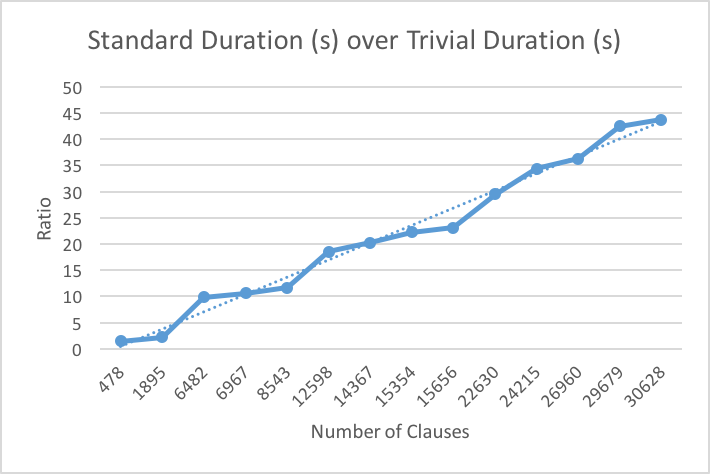
\includegraphics{png/standarddurationovertrivialduration.png}
\end{CenteredBox}
\end{figure}

\subsection{Size of Result}
The standard scheme does produce significantly smaller results than the trivial scheme. The relationship is similar to the ratio discussed in the time taken to convert. We look at the ratio of the size of the trivial scheme result over the size of the standard scheme result. In the smallest cases the standard scheme is at least four to five times smaller but can be as much as two hundred times smaller for larger problems. Again there is a linear relationship between the number of clauses and this ratio. As the number of clauses doubles, the ratio of trivial size over standard size doubles too, shown in the graph~\ref{trivialsizeoverstandardsize}.

\begin{figure}[h]
\caption{Ratio of trivial over standard duration}
\label{trivialsizeoverstandardsize}
\begin{CenteredBox}
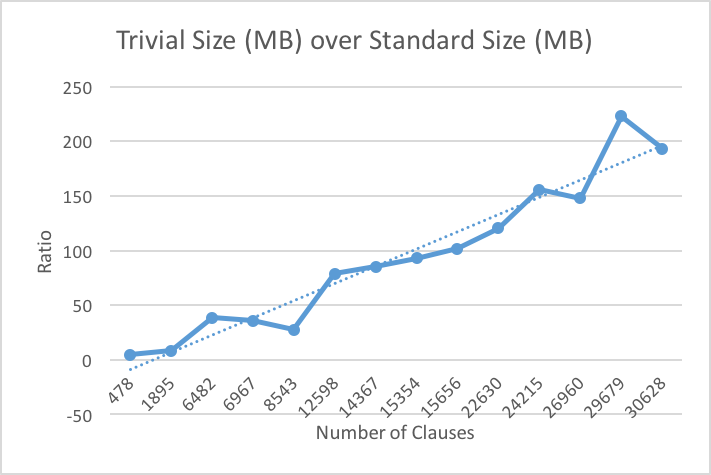
\includegraphics{png/trivialsizeoverstandardsize.png}
\end{CenteredBox}
\end{figure}

Given that this implementation of the standard dependency scheme misses some dependencies the correct file size is slightly higher but not enough to break this relationship.

\subsection{Time to Solve} \label{tvsstdsolve}
The hope is that the smaller problems are faster for iProver to solve and that this speed improvement outweighs the deficit introduced by the longer conversion time. This proved to be harder to show but can be loosely inferred from a single result. The problem \texttt{s27\_d5\_u-shuffled} is the smallest problem in the harder data set with 478 clauses. Using the trivial scheme took 0.015 seconds to convert to \gls{epr} with an output file-size of 117 Kilobytes and using the standard scheme took 0.021 seconds with an output of 26 Kilobytes. However, iProver took only 147.12 seconds to solve the standard result but had not solved the trivial result after an hour of processing. This shows that the extra time taken to convert using the standard dependency scheme is vastly outweighed by the time taken to solve in iProver on sufficiently large problems. To test this inference further the same test was carried out using the easy set of benchmarks but the difference here was negligible on the easy problems with only a hundred clauses.

\section{Comparison Against a Direct QBF Solver}
As mentioned to in section~\ref{eprnexptime}, in theory solving \gls{epr} is slower than solving the \gls{qbf} directly. The results agreed with this theory. Solving via converting with \textit{qbftoepr} and solving the \gls{epr} with iProver was approximately an order of magnitude slower than solving the problem directly with DepQBF. This is shown in the graph~\ref{depqbfvsqbftoeprgraph} with the full results in appendix~\ref{depqbfvsqbftoepr}.

\begin{figure}[h]
\caption{DepQBF vs. \textit{qbftoepr} time}
\label{depqbfvsqbftoeprgraph}
\begin{CenteredBox}
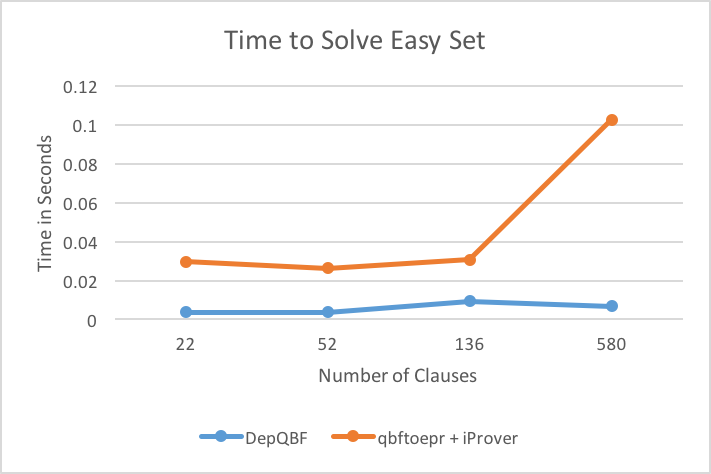
\includegraphics{png/depqbfvsqbftoepr.png}
\end{CenteredBox}
\end{figure}

\section{Comparison Against an EPR Converter}
The trivial dependency scheme is used throughout these tests as it is the only scheme implemented in qbf2epr so it is used when testing \textit{qbftoepr} to give a better comparison. Since the two converters give identical output (aside from differences in variable names) only the conversion time is examined as the differences in time taken for iProver to solve the output would be negligible. The results show in the graph~\ref{qbftoeprvsqbf2eprhard} that the conversion time of qbf2epr increases linearly with the number of clauses whereas \textit{qbftoepr} increases with the square of the number of clauses. This means that as the problem size increases the algorithmic inefficiencies in \textit{qbftoepr} lead to a significant time difference, up to 20 times slower in the largest problem. However on the smaller problem sets \textit{qbftoepr} is almost an order of magnitude faster than qbf2epr (shown in graph~\ref{qbftoeprvsqbf2epreasy}) suggesting that if it were improved it could be significantly faster on larger problem sets.

\begin{figure}[h]
\caption{\textit{qbftoepr} vs. qbf2epr hard benchmark}
\label{qbftoeprvsqbf2eprhard}
\begin{CenteredBox}
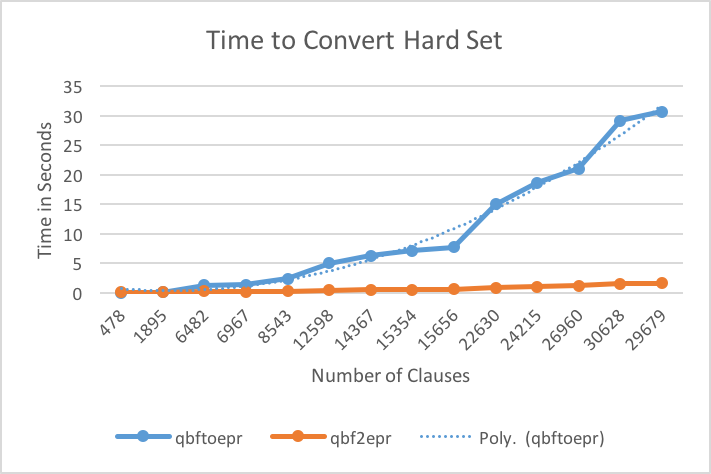
\includegraphics{png/qbftoeprvsqbf2eprhard.png}
\end{CenteredBox}
\end{figure}

\begin{figure}[h]
\caption{\textit{qbftoepr} vs. qbf2epr easy benchmark}
\label{qbftoeprvsqbf2epreasy}
\begin{CenteredBox}
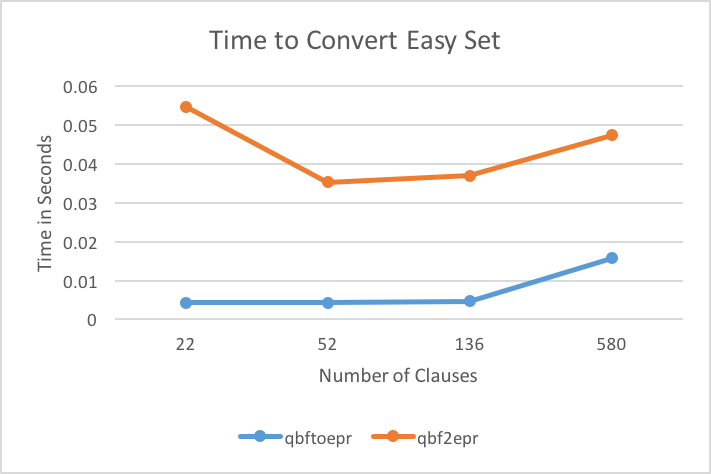
\includegraphics{png/qbftoeprvsqbf2epreasy.png}
\end{CenteredBox}
\end{figure}
